\documentclass[tikz,border=2mm]{standalone}
\usepackage{xcolor}
\begin{document}
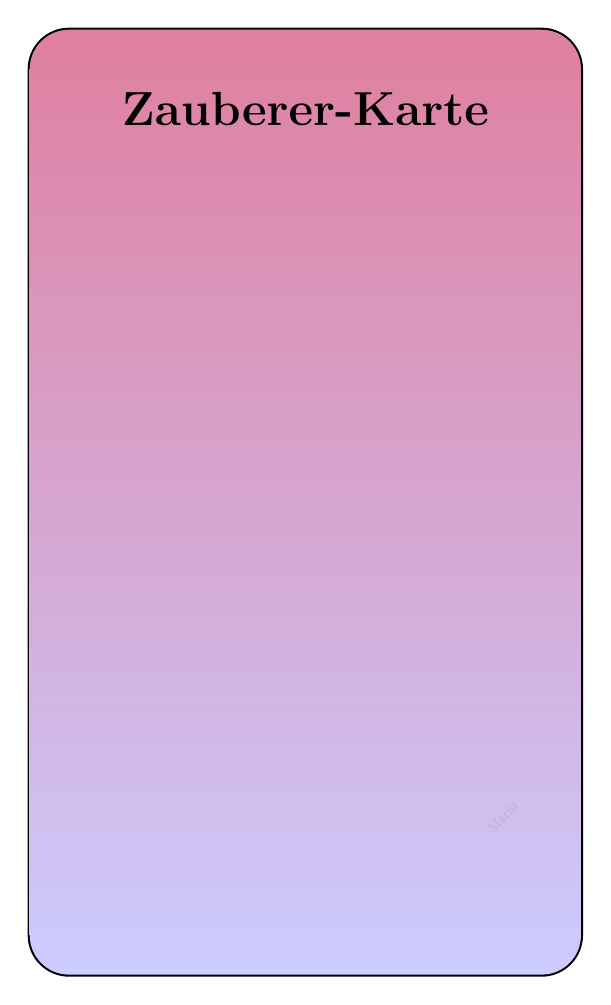
\begin{tikzpicture}[x=1mm,y=1mm]
  % Rahmen mit abgerundeten Ecken
  \draw[rounded corners=5mm, line width=1.5pt, black] (0,0) rectangle (70,120);
  
  % Hintergrund mit Farbverlauf (magischer Effekt)
  \shade[rounded corners=5mm, bottom color=blue!20, top color=purple!50] (0,0) rectangle (70,120);
  
  % Titel der Karte
  \node at (35,110) {\fontsize{16}{18}\selectfont\textbf{Zauberer-Karte}};
  
  % Zentrales Designelement (großer Stern)
  \node at (35,70) {\fontsize{40}{42}\selectfont$\bigstar$};
  
  % Verstecktes Easter Egg (leicht transparent)
  \node[rotate=45, opacity=0.1, scale=0.5] at (60,20) {Mario};
\end{tikzpicture}
\end{document}
